%!TEX root = index.tex
\chapter[Introdução]{Introdução}
\label{chap:introducao}
\section{Contextualização do trabalho}
\label{cha:contexto}

Neste capítulo será mostrado o contexto que a empresa, chamada de BC, na qual o autor realizou o trabalho de conclusão de curso estava inserida.

A empresa BeeConnect (BC), faz parte de um grupo de tecnologia chamado TM. A história da holding Techmob (TM) começa no ano de 2010 no qual um aluno da Engenharia de Produção da Escola Politécnica da USP criou uma empresa chamada Best Cool and Fun Games (BCFG). Tal empresa criou diversos aplicativos de sucesso tais como Bunny Shooter e Ant Smasher, este último atingiu recentemente mais 150 milhões de downloads na \textit{Play Store}, loja de aplicativos da \textit{Google}, como mostrado na \autoref{fig:antsmasherGooglePlay}. 

\begin{figure}[H]
\caption{Ant Smasher na loja de aplicativos para o sistema operacional Android}
\centerline{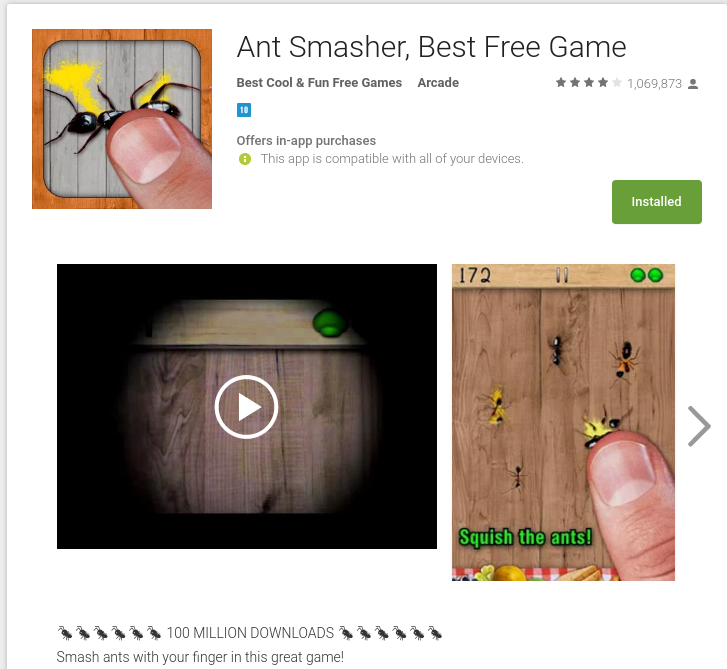
\includegraphics[scale=0.5]{img/antsmasherGooglePlay}}
\label{fig:antsmasherGooglePlay}
\caption* {Fonte: https://play.google.com/store/apps/details?id=com.bestcoolfungames.antsmasher}
\end{figure}

Grande parte do fluxo de receita da BCFG vinha através de publicidade em seus jogos. Como mostra a \autoref{fig:antsmasheriOS}
\begin{figure}[H]
\caption{Banner de propaganda no Ant Smasher para iOS}
\centerline{
\includegraphics[scale=0.5]{img/antsmasheriOS}}
\label{fig:antsmasheriOS}
\caption* {Fonte: Website Revmob - https://www.revmobmobileadnetwork.com/site}
\end{figure}

Na época haviam poucas redes de propaganda que proviam um serviço de baixa qualidade para os desenvolvedores de aplicativos. Sabiamente, o fundador da BCFG resolveu criar sua própria rede de propagandas, para tirar proveito desse mercado. Surgiu então em 2011 a Revmob (RM), que rapidamente se tornou a maior rede de propagandas para aparelhos móveis da América Latina, mesmo não tendo focado tanto no mercado brasileiro. Em 2015 a empresa buscou dar mais atenção ao Brasil buscando mais anunciantes e desenvolvedores de aplicativos brasileiros. Para alinhar com essa estratégia fez uma versão em português do \textit{website} da empresa como mostra a \autoref{fig:screenshotSiteRev}.

\begin{figure}[H]
\caption{Website RevMob para o Brasil}
\centerline{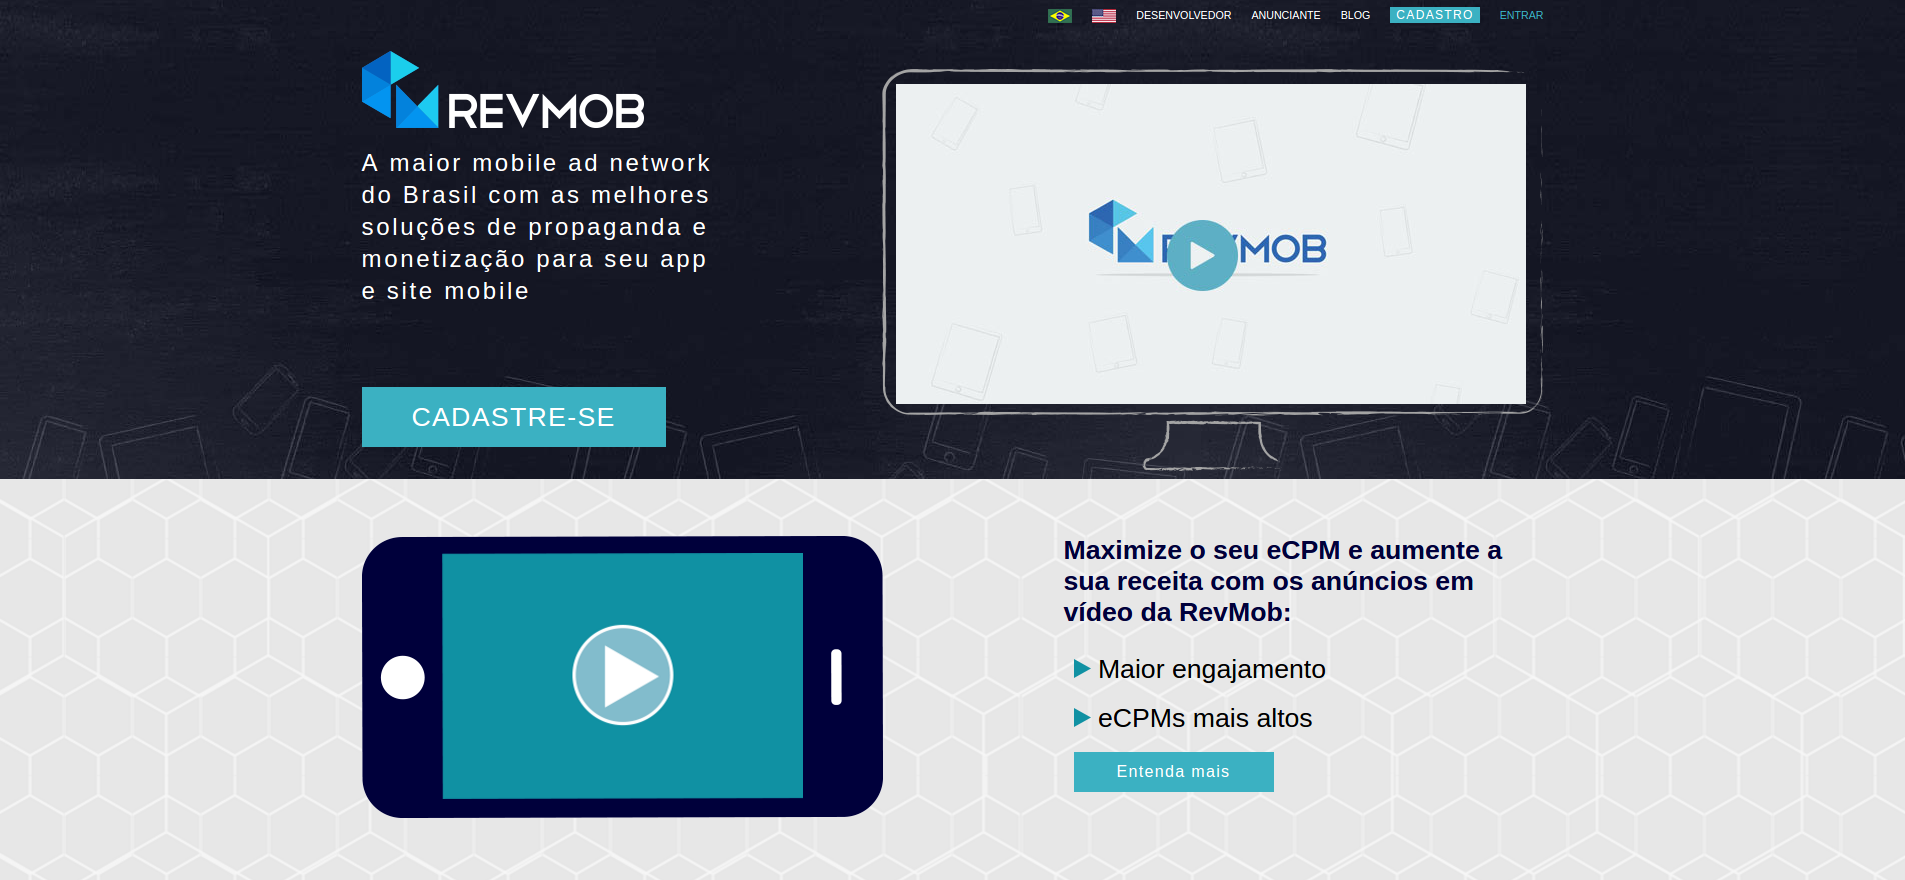
\includegraphics[width=0.8\textwidth]{img/screenshotSiteRev}}
\label{fig:screenshotSiteRev}
\caption* {Fonte: Website Revmob - https://www.revmobmobileadnetwork.com/site}
\end{figure}

O mercado de redes de anúncio cresceu rapidamente e se tornou muito competitivo. As grandes vantagens competitivas nesse mercado são:
\begin{itemize}
\item Servir rapidamente o anúncio, baixa latência, em questão de menos de 100 milissegundos.
\item Saber estimar as taxas de conversão de um anúncio. Para cada vez que o anúncio aparecer qual a chance dele ser clicado, e para cada clique qual a chance do aplicativo ser instalado.
\item Saber aumentar as taxas de conversão de uma propaganda. Geolocalização precisa e saber as informações da pessoa para o qual o anúncio está sendo mostrado aumentam bastante as taxas de conversão.
\end{itemize}

O desafio da latência foi resolvido através de uma reestruturação dos sistemas e de reescrita do código. Para endereçar o desafio da estimativa das taxas de conversão foi necessária a criação de uma nova empresa chamada Beluga, criada em 2014. As soluções de Big Data eram demasiadamente caras e de difícil integração com o sistema da Revmob. E sobre o aumento das taxas de conversão a Revmob decidiu focar na questão da geolocalização precisa, através da tecnologia de beacons, o que culminou no nascimento da empresa Beeconnect em 2015, que será o foco desse trabalho de formatura.

\section{Contexto da Beeconnect}
\label{cha:contexto_da_beeconnect}
A Beeconnect surgiu para externalizar os conhecimentos obtidos com as demais empresas do grupo Techmob. A empresa nasceu com 4 pessoas com a supervisão de um membro do Board da Techmob.

A empresa queria tirar proveito da tecnologia de beacons que estava na moda em 2015, porém poucos no Brasil tinham ouvido falar, o que poderia ser uma vantagem competitiva. O beacon é um aparelho que utiliza a tecnologia \textit{Bluetooth Low Energy} ou BLE que pode ser utilizado para geolocalização interna com uma ótima precisão, superando em muito o GPS para locais internos como Shoppings, por exemplo.

A equipe fez diversas análises de como os beacons estavam sendo utilizados no exterior e descobriu diversas aplicações em lugares diversos como shoppings, vide \autoref{fig:beaconShopping}, aeroportos, hospitais, hotéis e museus. O time estava ansioso para testar essa tecnologia em alguma aplicação mas ainda não tinha ideia do que fazer.

\begin{figure}[H]
\caption{Aplicação de beacon em shopping}
\centerline{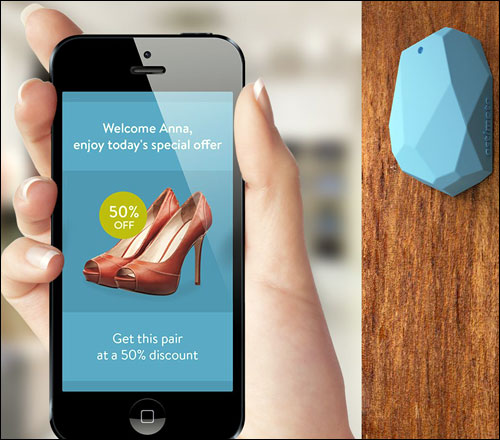
\includegraphics[scale=0.5]{img/beaconShopping}}
\label{fig:beaconShopping}
\caption* {Fonte: Material de marketing da Estimote - fornecedora de beacons}
\end{figure}

Até que um dos membros da equipe utilizou um contato que trabalhava em um grande shopping da capital paulista e agendou uma reunião para apresentar a tecnologia de beacons e o valor que a Beeconnect conseguiria gerar para eles. Dado o histórico da Techmob com propagandas em dispositivos móveis o time acabou optando por criar um aplicativo que disparava uma notificação assim que o celular entrasse em um raio de meio metro do beacon. Rapidamente a equipe desenvolveu  um produto que serviria para mandar propagandas geolocalizadas, trabalhando cerca de 16 horas por dia por uma semana, que consistia em:
\begin{itemize}
\item Um aplicativo para iOS que possuía um SDK (basicamente um software) que permitia a comunicação com beacons.
\item Um servidor que fazia a comunicação com o aplicativo e gravava todas as informações de distância do celular em relação ao beacon e enviava uma propaganda para o aplicativo.
\end{itemize}

Porém na apresentação para o Shopping a equipe sequer apresentou o produto desenvolvido dado que o cliente claramente não parecia estar interessado com a ideia de publicidade móvel feita de dessa maneira.

Todos ficaram muito frustrados com o tempo perdido e a sensação de que haveria um jeito melhor de ter desenvolvido o projeto sem ter gasto esforços com tarefas desnecessárias ou que não tinham um valor claro a ser gerado.

A equipe então começou a vender a ideia do que a Beeconnect poderia fazer e criar o produto junto com o cliente. Basicamente utilizou-se o processo de vender apresentações em slides para validar a ideia de que uma ferramenta de geolocalização precisa tem valor. Foram feitas reuniões com diversos tipos de clientes: hospitais, hotéis, construtoras, concessionárias e varejistas. Após essas reuniões o foco da empresa ficou mais claro. O varejo pareceu ser a opção mais rentável pois trata-se de um mercado gigantesco e que tem uma necessidade de saber mais sobre os consumidores.

Após acumular alguns varejistas interessados ficou evidente a necessidade da criação de um produto para ser testado. A pressão por resultados fez até o autor abrir mão da graduação na Escola Politécnica para trabalhar cerca de 14 horas por dia para liderar o desenvolvimento tanto de um servidor quanto de um aplicativo para smartphones \textit{Android}. Dado o aparente interesse dos varejistas por essa tecnologia a Beeconnect realizou mais contratações para auxiliar tanto em vendas quanto no desenvolvimento de software.

O produto criado foi um aplicativo de descontos chamado iShop, que utilizava a tecnologia de beacons para gerar um cupom de desconto somente na loja física cadastrada. O funcionamento do aplicativo basicamente consistia em quatro etapas conforme mostrado na \autoref{fig:explicacaoBeeconnect}:

\begin{figure}[H]
\caption{Funcionamento app Beeconnect}
\centerline{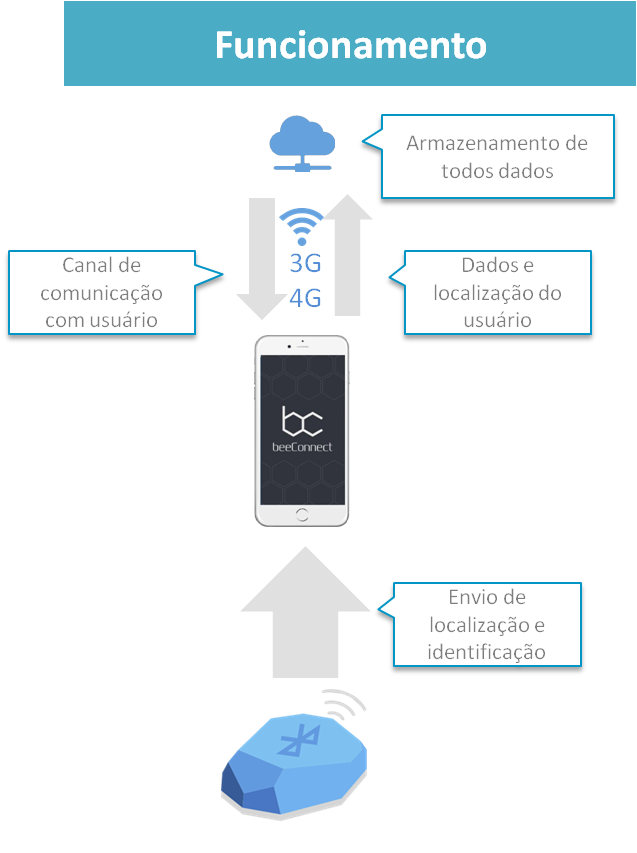
\includegraphics[scale=0.75]{img/explicacaoBeeconnect}}
\label{fig:explicacaoBeeconnect}
\caption* {Fonte: Material de marketing da Beeconnect}
\end{figure}

\begin{itemize}
\item Comunicação do celular com o beacon: O beacon é um aparelho passivo, ou seja, ele só emite um sinal mandando três informações: \textit{UUID}, \textit{Major} e \textit{Minor}. O \textit{UUID} é o identificador único universal, trata-se de um número hexadecimal de trinta e dois dígitos que para o caso dos beacons tem como propósito identificar uma rede de beacons. Já o \textit{Major} e \textit{Minor} são números inteiros que variam de 0 a 65535 que têm como objetivo identificar um beacon dentro da rede dele.
\item Interação do usuário com o aplicativo: com o aplicativo o usuário consegue ver as ofertas mais relevantes para ele, consultar as lojas mais próximas a ele e gerar cupons de desconto.
\item Comunicação do celular com o servidor: O aplicativo só funciona se o usuário estiver conectado a internet, seja por meio do 3G/4G ou via \textit{WiFi}. O servidor então manda para o celular as ofertas mais relevantes baseadas na localização do usuário enviada pelo celular. Além disso, o celular envia para o servidor qual beacon que ele está detectando para que o servidor decida ou não enviar uma notificação para o usuário.
\item Interação do varejista com a plataforma: Para o varejista foi criada uma plataforma, um site, ilustrado na \autoref{fig:plataforma_varejistas}, onde ele consegue gerenciar as informações e as promoções de cada loja. Tais dados são então salvos na base de dados e então disponibilizados para o aplicativo.
\end{itemize}

\begin{figure}[H]
\caption{Plataforma para Varejistas}
\centerline{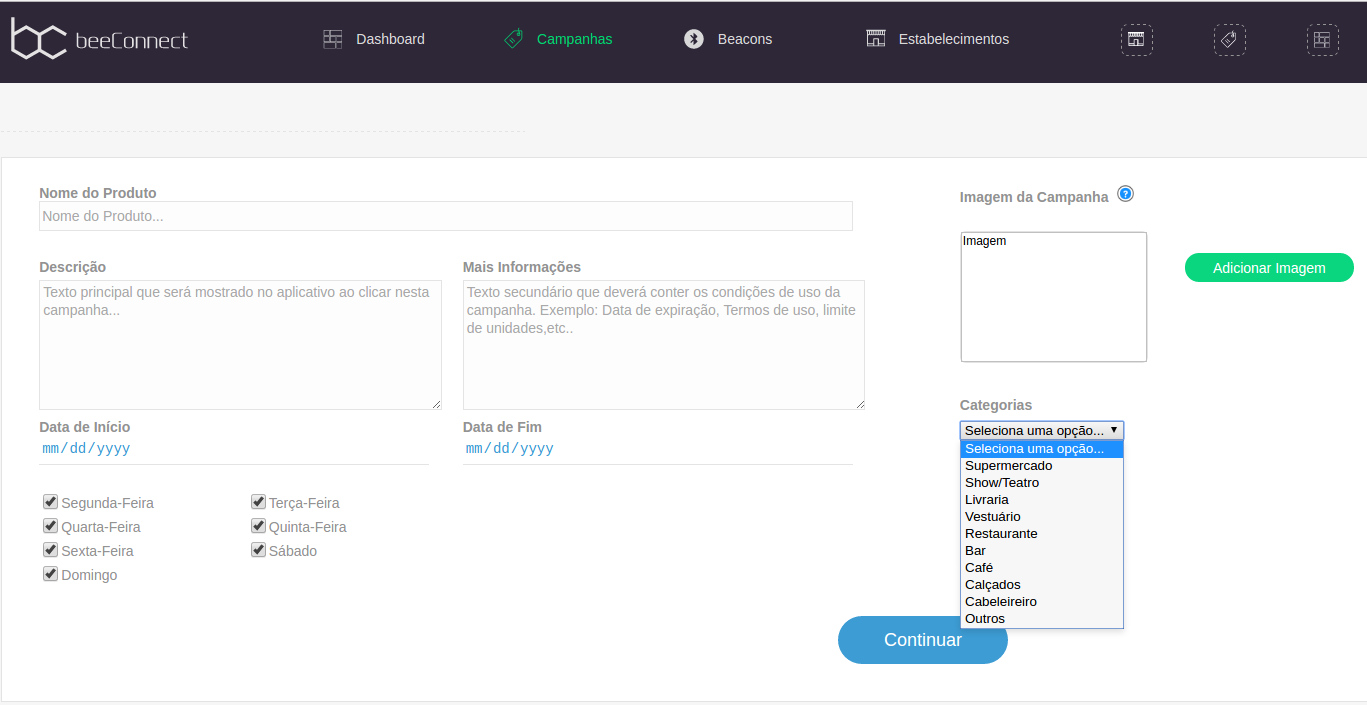
\includegraphics[scale=0.3]{img/plataforma_varejistas}}
\label{fig:plataforma_varejistas}
\caption* {Fonte: https://app.beeconnect.com.br/}
\end{figure}

O primeiro piloto para testar esse produto foi realizado no McDonald's localizado na Riviera de São Lourenço. Foram disponbilizadas cinco ofertas para o aplicativo, desde McOfertas até sobremesas e bebidas.
Houve a geração e utilização de alguns cupons no local, entretanto nada muito relevante. Todos os usuários que baixaram o aplicativo acharam muito simples e fácil de gerar o desconto, entretanto poucas pessoas o baixaram. A distância entre o local do piloto e o escritório da Techmob deixava inviável um acompanhamento de perto. 

Além disso, por motivos estratégicos a matriz do McDonald's do Brasil pediu para que o piloto fosse cancelado. E no meio de toda essa turbulência, o advogado da Techmob sugeriu que o nome do aplicativo fosse mudado porque dificilmente algum nome de marca com "i" como prefixo seria registrado, pois já é praticamente um consenso que esse prefixo remete aos produtos e serviços da marca \textit{Apple}. Assim, a equipe decidiu registrar a marca Beeconnect e utilizá-la como nome do aplicativo também. Foi necessária também uma reformulação no design do aplicativo para que ficasse condizente com a marca.

Após tais insucessos e com muito esforço a empresa conseguiu fechar um piloto com o maior varejista da América Latina, o Grupo Pão de Açúcar. Foi realizado um piloto na loja dentro da sede da empresa. A promoção foi "Todas as cervejas premium com 50\% de desconto". O resultado foi um sucesso. Vários funcionários baixaram o aplicativo na hora e conseguiram utilizar o desconto sem problemas. O resultado do piloto foi um contrato assinado no qual seriam implementados beacons em todas as lojas de formato de proximidade premium, chamadas de Minuto Pão de Açúcar, no estado de São Paulo.

Após a implementação dos beacons em todas as Minuto Pão de Açúcar, esperou-se um resultado condizente com o esforço. Infelizmente tal resultado não veio. A pressão resultados do board da Techmob veio. A holding havia gasto cerca de R\$500.000 reais até então.

\section{Definição do problema}
\label{cha:definição_do_problema}
A Beeconnect estava prestes a ser um projeto engavetado. A empresa já gastara cerca de meio milhão de reais no decorrer de um ano, entre os seus principais custos envolvem os recursos humanos. Dado que o time dessa startup era muito bem qualificado, praticamente todos os integrantes do time eram engenheiros formados ou estudantes de engenharia pela Escola Politécnica, e que havia outras frentes da Techmob que também necessitavam de recursos, o Conselho da holding começou a pressionar a Beeconnect para gerar resultados, caso contrário, eles iriam começar a desmontar o time para suprirem outras áreas da holding.

O principal problema é que a startup ainda não sabia se possuía um modelo de negócio sustentável e que gera valor para seus clientes. A empresa encontrava-se em momento no qual tinha um grande primeiro cliente, que entretanto estava em modo de testes, ou seja, não estava pagando.
Todo o negócio da empresa começou sem ter um planejamento ou alguma base teórica para fomentar um desenvolvimento mais sólido do negócio. Tudo isso foi agravado pelo fato da empresa ter crescido em número de funcionários sem ter provado o modelo de negócio, o que acabou inflando os custos.

A empresa sequer tinha feito um Canvas de Modelo de Negócio para que todos da equipe conseguissem ter uma visão geral do projeto e poderem opinar e iterar em cima do modelo. Dessa forma pelo fato da Beeconnect ter começado mal estruturada, praticamente um ano havia se passado e ainda não estava claro se a empresa deveria perseverar em seu modelo de negócio, pivotar para outro tipo de negócio ou simplesmente fechar a empresa e realocar os recursos para outras áreas.

Além disso, faltavam mais lojas para validar a proposta de valor da Beeconnect no lado dos varejistas assim como faltavam mais usuários para verificar se eles enxergavam valor no aplicativo. A Beeconnect encontrava-se no clássico problema do "Ovo e da Galinha", no qual os varejistas reclamavam que a base de usuários do aplicativo era muito pequena e só entrariam quando a base fosse maior. No caso dos usuários muitos faziam reclamações sobre o baixo número de lojas que os interessavam.

\section[Objetivos]{Objetivos}
\label{chap:objetivos}
Dado o problema apresentado fica evidente que a Beeconnect precisa ser estruturada de modo a virar uma máquina de testar hipóteses para que a startup itere o mais rápido possível de forma a encontrar o seu modelo de negócio.
A reestruturação deve visar responder se a Beeconnect gera valor para seus clientes, tanto para os varejistas quanto para os usuários do aplicativo. 

O grande indicador de que os lojistas estão vendo valor no aplicativo, para a Beeconnect e para a holding Techmob é o fato dos varejistas estarem dispostos a pagar pelo serviço disponibilizado. Uma vez que houver tal fluxo de receita para o caixa da empresa a holding poderá aumentar seu investimento de forma a captar mais varejistas e usuários para o aplicativo, com tal ciclo positivo a tendência é ficar cada vez mais fácil de trazer mais usuários e lojas. Assim a empresa gastará cada vez menos proporcionalmente a receita em marketing, uma vez que o aplicativo passará a ser mais conhecido, crescendo organicamente e com margens de lucro cada vez melhores. 

O modelo a ser seguido deverá seguir a literatura ligada ao empreendedorismo, principalmente a de \citeonline{leanstartup}, \citeonline{businessmodel} e \citeonline{startupowners}

\section{Justificativa}
\label{cha:justificativa}
Para o autor a importância do tema desse trabalho é imensa dado que a Beeconnect tem sido basicamente a vida dele durante o último ano. Foram madrugadas trabalhando, noites mal dormidas, finais de semana perdidos, graduação postergada para que a Beeconnect saísse do papel e conquistasse o varejo físico brasileiro, talvez mundial.

Para a Techmob verifica-se a relevância de utilizar os métodos propostos pela literatura e como isso pode fazer diferença na hora de começar novas empresas bem como tal iniciativa pode trazer economias para testar novas hipóteses.

Dado que o espírito empreendedor está cada vez mais forte dentro da Escola Politécnica da Universidade de São Paulo. O trabalho aqui apresentado mostra a relevância do ensino de tais métodos de empreendedorismo, para que as futuras startups criadas por politécnicos não tenham um início tão turbulento quanto a empresa analisada neste trabalho. E caso a startup também saia mal estruturada assim como a Beeconnect que esse trabalho de conclusão de curso seja um material de referência para auxiliar empresas que estão passando por um processo de reestruturação.

Para a sociedade a importância é mostrar que no empreendedorismo não basta ter uma boa ideia, parece que todo mundo quer fazer um aplicativo. É necessário que essa ideia seja bem estruturada e o mais importante, que ela seja validada o mais rápido possível. É importante apresentar que o mundo empreendedor não é glamouroso como se mostram nos filmes e nas revistas, que não é nada fácil construir o próximo \textit{Facebook} ou \textit{Google}. É preciso demonstrar que a escolha de empreender tem que vir com a vontade de passar por dificuldades, por momentos de estresse. O empreendedor tem que ser resiliente. 

\section{Estrutura do Trabalho}
\label{cha:estrutura_do_trabalho}
O trabalho de formatura foi estruturado conforme apresentado abaixo:

No Capítulo 1 o autor introduz a origem da Beeconnect, insere o leitor no contexto da empresa, apresenta a definição do problema que startup encontrava, propõe os objetivos do trabalho de conclusão de curso, assim como menciona a justificativa do trabalho demonstrando-se sua relevância.

O Capítulo 2 apresenta a bibliografia utilizada pelo autor para que o trabalho pudesse ser desenvolvido. Foram apresentados os conceitos da Startup Enxuta, Desenvolvimento de Clientes, Métricas Pirata, Canvas de Modelo de Negócio e Canvas de Proposição de Valor.

No Capítulo 3 o autor insere a metodologia utilizada durante o desenvolvimento do trabalho do projeto de modo a atingir os objetivos estabelecidos previamente.

O Capítulo 4 apresenta os testes realizados pelo autor bem como seus resultados e análise dos mesmos.

O Capítulo 5 finaliza o trabalho com uma discussão sobre toda jornada realizada bem como uma reflexão sobre as lições aprendidas no decorrer de todo o processo.